\documentclass{article}
% Change "article" to "report" to get rid of page number on title page
\usepackage{amsmath,amsfonts,amsthm,amssymb}
\usepackage{setspace}
\usepackage{Tabbing}
\usepackage{fancyhdr}
\usepackage{lastpage}
\usepackage{extramarks}
\usepackage{chngpage}
\usepackage{soul,color}
\usepackage{graphicx,float,wrapfig}
\usepackage{multirow}

% In case you need to adjust margins:
\topmargin=-0.45in      %
\evensidemargin=0in     %
\oddsidemargin=0in      %
\textwidth=6.5in        %
\textheight=9.0in       %
\headsep=0.25in         %

% Homework Specific Information
\newcommand{\hmwkTitle}{Weekly Report IV}
\newcommand{\hmwkClass}{}
\newcommand{\hmwkAuthorName}{Donglai\ Wei}


% Setup the header and footer
\pagestyle{fancy}                                                       %
\lhead{\hmwkAuthorName}                                                 %
\rhead{\firstxmark}                                                     %
\lfoot{\lastxmark}                                                      %
\cfoot{}                                                                %
\rfoot{Page\ \thepage\ of\ \pageref{LastPage}}                          %
\renewcommand\headrulewidth{0.4pt}                                      %
\renewcommand\footrulewidth{0.4pt}                                      %

% This is used to trace down (pin point) problems
% in latexing a document:
%\tracingall

%%%%%%%%%%%%%%%%%%%%%%%%%%%%%%%%%%%%%%%%%%%%%%%%%%%%%%%%\begin{enumerate}

% Some tools
\newcommand{\enterProblemHeader}[1]{\nobreak\extramarks{#1}{#1 continued on next page\ldots}\nobreak%
                                    \nobreak\extramarks{#1 (continued)}{#1 continued on next page\ldots}\nobreak}%
\newcommand{\exitProblemHeader}[1]{\nobreak\extramarks{#1 (continued)}{#1 continued on next page\ldots}\nobreak%
                                   \nobreak\extramarks{#1}{}\nobreak}%

\newlength{\labelLength}
\newcommand{\labelAnswer}[2]
  {\settowidth{\labelLength}{#1}%
   \addtolength{\labelLength}{0.25in}%
   \changetext{}{-\labelLength}{}{}{}%
   \noindent\fbox{\begin{minipage}[c]{\columnwidth}#2\end{minipage}}%
   \marginpar{\fbox{#1}}%

   % We put the blank space above in order to make sure this
   % \marginpar gets correctly placed.
   \changetext{}{+\labelLength}{}{}{}}%

\setcounter{secnumdepth}{0}
\newcommand{\homeworkProblemName}{}%
\newcounter{homeworkProblemCounter}%
\newenvironment{homeworkProblem}[1][Problem \arabic{homeworkProblemCounter}]%
  {\stepcounter{homeworkProblemCounter}%
   \renewcommand{\homeworkProblemName}{#1}%
   \section{\homeworkProblemName}%
   \enterProblemHeader{\homeworkProblemName}}%
  {\exitProblemHeader{\homeworkProblemName}}%

\newcommand{\problemAnswer}[1]
  {\noindent\fbox{\begin{minipage}[c]{\columnwidth}#1\end{minipage}}}%

\newcommand{\problemLAnswer}[1]
  {\labelAnswer{\homeworkProblemName}{#1}}

\newcommand{\homeworkSectionName}{}%
\newlength{\homeworkSectionLabelLength}{}%
\newenvironment{homeworkSection}[1]%
  {% We put this space here to make sure we're not connected to the above.
   % Otherwise the changetext can do funny things to the other margin

   \renewcommand{\homeworkSectionName}{#1}%
   \settowidth{\homeworkSectionLabelLength}{\homeworkSectionName}%
   \addtolength{\homeworkSectionLabelLength}{0.25in}%
   \changetext{}{-\homeworkSectionLabelLength}{}{}{}%
   \subsection{\homeworkSectionName}%
   \enterProblemHeader{\homeworkProblemName\ [\homeworkSectionName]}}%
  {\enterProblemHeader{\homeworkProblemName}%

   % We put the blank space above in order to make sure this margin
   % change doesn't happen too soon (otherwise \sectionAnswer's can
   % get ugly about their \marginpar placement.
   \changetext{}{+\homeworkSectionLabelLength}{}{}{}}%

\newcommand{\sectionAnswer}[1]
  {% We put this space here to make sure we're disconnected from the previous
   % passage

   \noindent\fbox{\begin{minipage}[c]{\columnwidth}#1\end{minipage}}%
   \enterProblemHeader{\homeworkProblemName}\exitProblemHeader{\homeworkProblemName}%
   \marginpar{\fbox{\homeworkSectionName}}%

   % We put the blank space above in order to make sure this
   % \marginpar gets correctly placed.
   }%

%%%%%%%%%%%%%%%%%%%%%%%%%%%%%%%%%%%%%%%%%%%%%%%%%%%%%%%%%%%%%



%%%%%%%%%%%%%%%%%%%%%%%%%%%%%%%%%%%%%%%%%%%%%%%%%%%%%%%%%%%%%
% Make title
\title{\vspace{0.3in}\textmd{\textbf{\hmwkTitle}}}
\date{2010.5.11}
\author{\textbf{\hmwkAuthorName}}
%%%%%%%%%%%%%%%%%%%%%%%%%%%%%%%%%%%%%%%%%%%%%%%%%%%%%%%%%%%%%

\begin{document}
\begin{spacing}{1.1}
\maketitle

\section{0)Understanding Concentration parameter}
\subsection{I)DPmixture}
Concentration parameter: $\alpha$ \\
$\mathcal{F}([z])=\sum_{c=1}^{K}[\frac{DN_{c}}{2}log\pi+\frac{D}{2}log\frac{\xi_{c}}{\xi_{0}}log det(B_{c})
-\frac{\eta_{0}}{2}log det(B_{0})-log \frac{\Gamma_{D}(\frac{\eta_{c}}{2})}{\Gamma_{D}(\frac{\eta_{0}}{2})}$
\underline{ $ -log(\Gamma(N_{c}))-log \alpha]+log \frac{\Gamma(N+\alpha)}{\Gamma(\alpha)}$}\\ \\
\subsection{a)}
Given Ground Truth of $z^{*}$, $\mathcal{F}([z^{*}])$ is a function of $\alpha$:\\
$ \frac{\partial \mathcal{F}([z^{*}])}{\partial \alpha}=\Psi(N+\alpha)-\Psi(\alpha)-\dfrac{K}{\alpha}$
\begin{figure}[h] 
  \begin{minipage}[b]{0.5\textwidth} 
    \centering 
    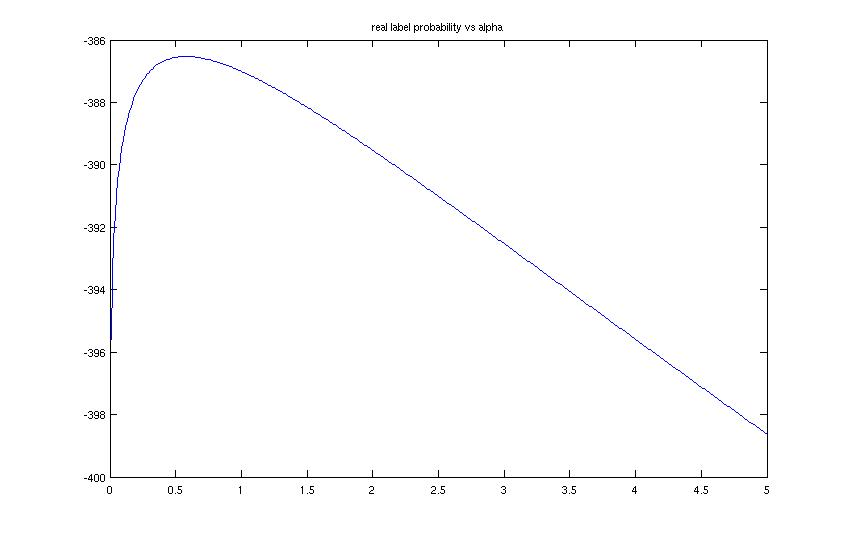
\includegraphics[width=3.5in,height=3in]{dp_alpha.jpg} 
    \caption{domain:0-5} 
    \label{fig:by:table} 
  \end{minipage}% 
  \begin{minipage}[b]{0.5\textwidth} 
    \centering 
    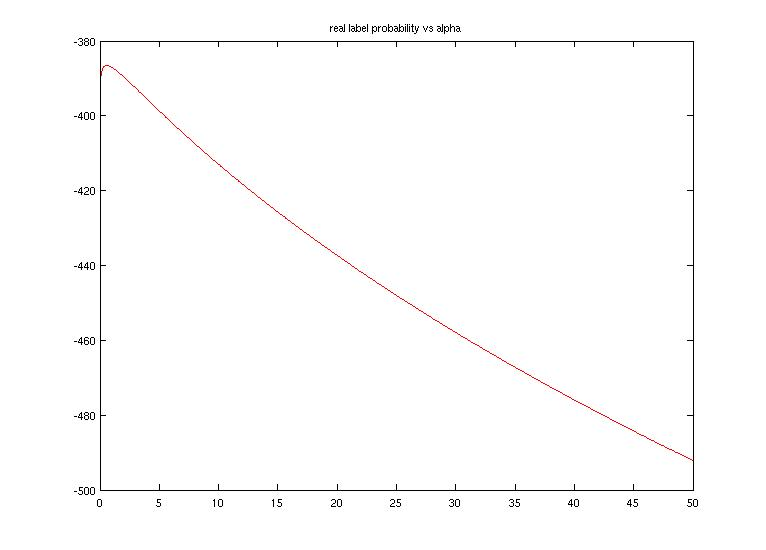
\includegraphics[width=3.5in,height=3in]{dd_alpha.jpg} 
    \caption{domain:0-50} 
    \label{fig:by:table}  
   \end{minipage}% 
\end{figure}


\subsection{b)}
Given $\alpha,\mathcal{F}([z])$\\
$=(Likelihood\ term)\sum_{c=1}^{K}[\frac{DN_{c}}{2}log\pi+\frac{D}{2}log\frac{\xi_{c}}{\xi_{0}}log det(B_{c})
-\frac{\eta_{0}}{2}log det(B_{0})-log \frac{\Gamma_{D}(\frac{\eta_{c}}{2})}{\Gamma_{D}(\frac{\eta_{0}}{2})}]$\\
$(Allocation\ term)-\sum_{c=1}^{K}[log(\Gamma(N_{c}))+log \alpha]$\\ \\
$(Constant\ term)+log \frac{\Gamma(N+\alpha)}{\Gamma(\alpha)}$

\begin{center}
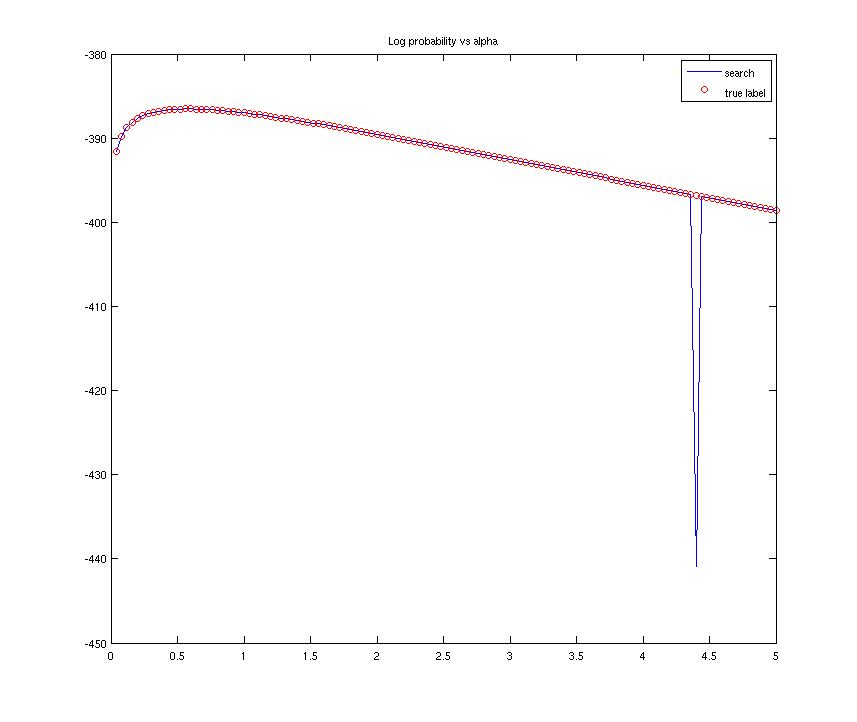
\includegraphics[width=5in,height=3in]{prob_alpha.jpg} \\
\end{center}


\subsection{II) HDP(multinomial)}


\begin{figure}[h] 
  \begin{minipage}[b]{0.5\textwidth} 
    \centering 
    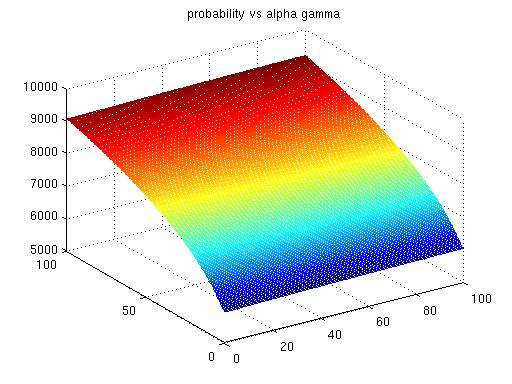
\includegraphics[width=3.5in,height=3in]{hyper.jpg} 
    \caption{Log-probability} 
    \label{fig:by:table} 
  \end{minipage}% 
  \begin{minipage}[b]{0.5\textwidth} 
    \centering 
    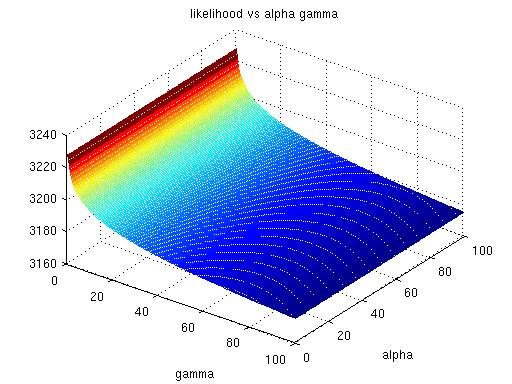
\includegraphics[width=3.5in,height=3in]{hyper2.jpg} 
    \caption{Likelihood term} 
    \label{fig:by:table}  
   \end{minipage}% 
\end{figure}

\section{1)Normal-Inverse Wishart}
$-log p(x|z,\lambda)$\\ =\\
(Likelihood)$ \sum_{k=1}^{K} [\frac{D n_{..k}}{2}log\pi+\frac{D}{2}log\frac{\xi_{k}}{\xi_{0}}+\frac{\eta_{k}}{2}log det(B_{k})-\frac{\eta_{0}}{2}log det(B_{0})
-log \frac{\Gamma_{D}(\frac{\eta_{k}}{2})}{\Gamma_{D}(\frac{\eta_{0}}{2})}]$
\\
+
\\
(Allocation:)$\underline{\sum_{j=1}^{J}\sum_{t=1}^{m_{j.}}[\frac{1}{m_{j.}}log \frac{\Gamma(n_{j..}+\alpha)}{\Gamma(\alpha)} -log(\Gamma(n_{jt.})-log \alpha]+
 \sum_{k=1}^{K} [\frac{1}{K}log \frac{\Gamma(T+\gamma)}{\Gamma(\gamma)} -log(\Gamma(m_{.k})-log \gamma]}$
\\ \\ \\
=\\
(t-term)$ \sum_{j=1}^{J}\sum_{t=1}^{m_{j.}}[\underline{\frac{1}{m_{j.}}log \frac{\Gamma(n_{j..}+\alpha)}{\Gamma(\alpha)} -log(\Gamma(n_{jt.})-log \alpha
+\frac{1}{J m_{j.}}log \frac{\Gamma(T+\gamma)}{\Gamma(\gamma)}]}$\\ \\
+(k-term)$\sum_{k=1}^{K} [\frac{n_{..k}D}{2}log\pi+\frac{D}{2}log\frac{\xi_{k}}{\xi_{0}}+\frac{\eta_{k}}{2}log det(B_{k})-\frac{\eta_{0}}{2}log det(B_{0})
-log \frac{\Gamma_{D}(\frac{\eta_{k}}{2})}{\Gamma_{D}(\frac{\eta_{0}}{2})}
-\underline{log(\Gamma(m_{.k})-log \gamma]}$\\ \\ \\ \\
=\\
(DP mixture of $z_{ji}$)$\sum_{k=1}^{K} [\frac{n_{..k}D}{2}log\pi+\frac{D}{2}log\frac{\xi_{k}}{\xi_{0}}+\frac{\eta_{k}}{2}log det(B_{k})-\frac{\eta_{0}}{2}log det(B_{0})
-log \frac{\Gamma_{D}(\frac{\eta_{k}}{2})}{\Gamma_{D}(\frac{\eta_{0}}{2})}
-log(\Gamma(n_{..k}))-log \gamma]$\\ \\
-(m term)$\sum_{k=1}^{K} log [\dfrac{\Pi_{j=1}^{J}(\Gamma(n_{j.k})}{\Gamma(n_{..k})}]-log\dfrac{\Pi_{k=1}^{K}\Gamma(m_{.k})}{\Gamma(T+\gamma)}-Tlog(\alpha)$\\ \\
+(constant)$\sum_{j=1}^{J}log \frac{\Gamma(n_{j..}+\alpha)}{\Gamma(\alpha)}+log \Gamma(\gamma)$


where:\\
$\xi_{k}=\xi_{0}+n_{..k}$\\
$m_{k}=\frac{n_{..k} \vec x_{(k_{jt_{ji}}=k)}+\xi_{0}m_{0}}{\xi_{k}}$\\
$\eta_{k}=\eta_{0}=n_{..k}$\\
$B_{k}=B_{0}+n_{..k}S_{k}+\frac{n_{..k}\xi_{0}}{\xi_{k}}(\vec x_{(k_{jt_{ji}}=k)}-m_{0})(\vec x_{(k_{jt_{ji}}=k)}-m_{0})^{T}$\\
$S_{k}: sample covariance$\\

\section{2)Dirichlet-Multinomial}
W:number of unique words\\ 
$n_{..k}^{w}$number of occurence of word w in dish k \\ \\
$-log p(x|z,\lambda)$\\ =\\
(Likelihood)$ \sum_{k=1}^{K} [log(\frac{\Gamma(n_{..k}+W\phi_{0})}{\Gamma(W\phi_{0})})+\sum_{w=1}^{W}log(\frac{\Gamma(\phi_{0})}{\Gamma(\phi_{0}+n_{..k}^{w})})]$
\\
+
\\
(Allocation:)$\underline{\sum_{j=1}^{J}\sum_{t=1}^{m_{j.}}[\frac{1}{m_{j.}}log \frac{\Gamma(n_{j..}+\alpha)}{\Gamma(\alpha)} -log(\Gamma(n_{jt.})-log \alpha]+
 \sum_{k=1}^{K} [\frac{1}{K}log \frac{\Gamma(T+\gamma)}{\Gamma(\gamma)} -log(\Gamma(m_{.k})-log \gamma]}$
\\ \\ \\
=\\
(t-term)$ \underline{log \frac{\Gamma(T+\gamma)}{\Gamma(\gamma)}+\sum_{j=1}^{J} \{log \frac{\Gamma(n_{j..}+\alpha)}{\Gamma(\alpha)}-\sum_{t=1}^{m_{j.}}[log(\Gamma(n_{jt.})+log \alpha
]\}}$\\ \\
+(k-term)$ \sum_{k=1}^{K} [log(\frac{\Gamma(n_{..k}+W\phi_{0})}{\Gamma(W\phi_{0})})+log(\Pi_{w=1}^{W}\frac{\Gamma(\phi_{0})}{\Gamma(\phi_{0}+n_{..k}^{w})})
-\underline{log(\Gamma(m_{.k})-log \gamma]}$\\ \\ 
=\\
(k-term)$ +\sum_{k=1}^{K} [log(\frac{\Gamma(n_{..k}+W\phi_{0})}{\Pi_{1}^{W}\Gamma(\phi_{0}+n_{..k}^{w})\Gamma(m_{.k})\Pi_{q=1}^{m_{.k}}\Gamma(n_{q.})})]$\\ 
(hyper-term)$-Tlog\alpha-Klog\gamma+Klog\frac{\Gamma(\phi_{0})^{W}}{\Gamma(W\phi_{0})}+log\Gamma(T+\gamma)$\\
(constant-term)$-log\Gamma(\gamma)+\sum_{j=1}^{J} log \frac{\Gamma(n_{j..}+\alpha)}{\Gamma(\alpha)}$
\\ \\


\subsection{Experiment}
$\alpha=0.5,\gamma=1.5$\\
\begin{figure}[h] 
  \begin{minipage}[b]{0.5\textwidth} 
    \centering 
    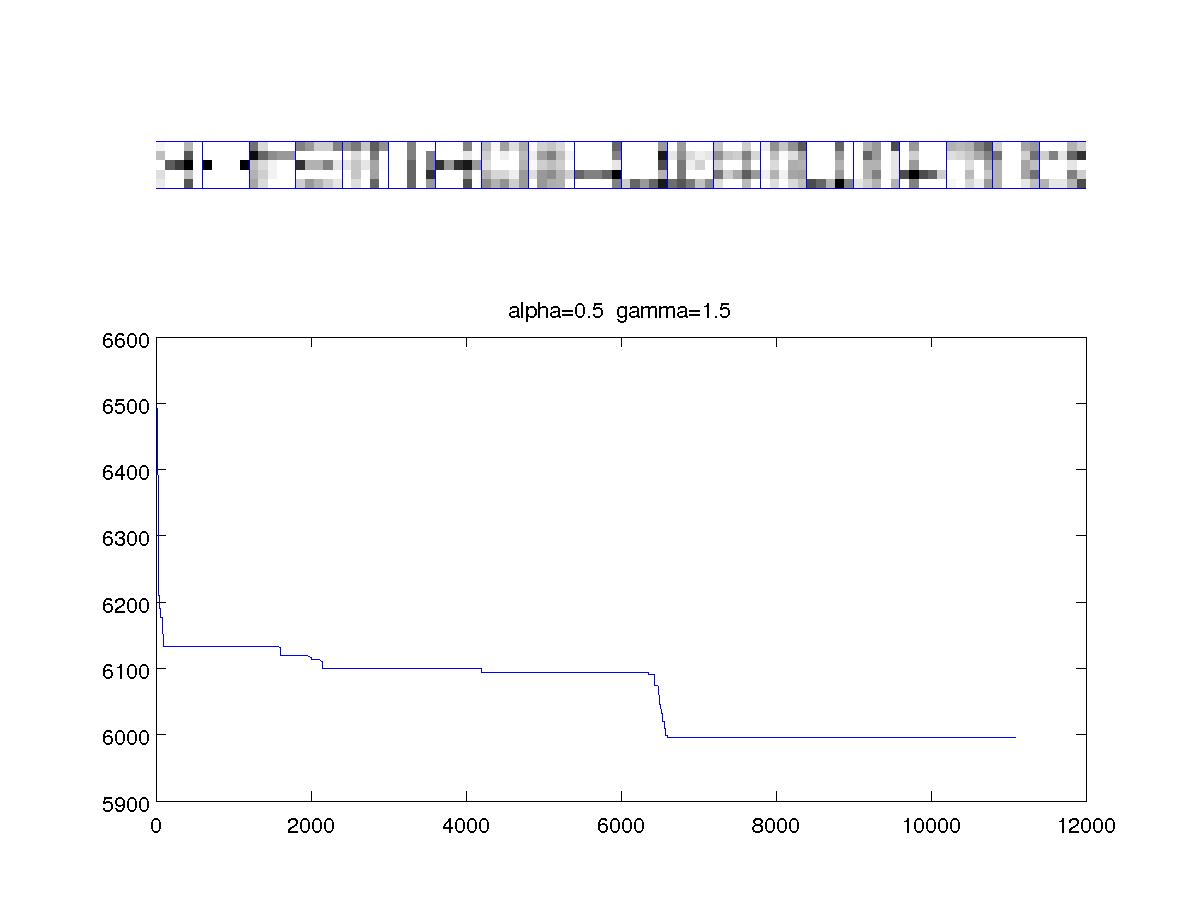
\includegraphics[width=3.5in,height=3in]{exp_me1.jpg} 
    \caption{ME result} 
    \label{fig:by:table} 
  \end{minipage}% 
  \begin{minipage}[b]{0.5\textwidth} 
    \centering 
    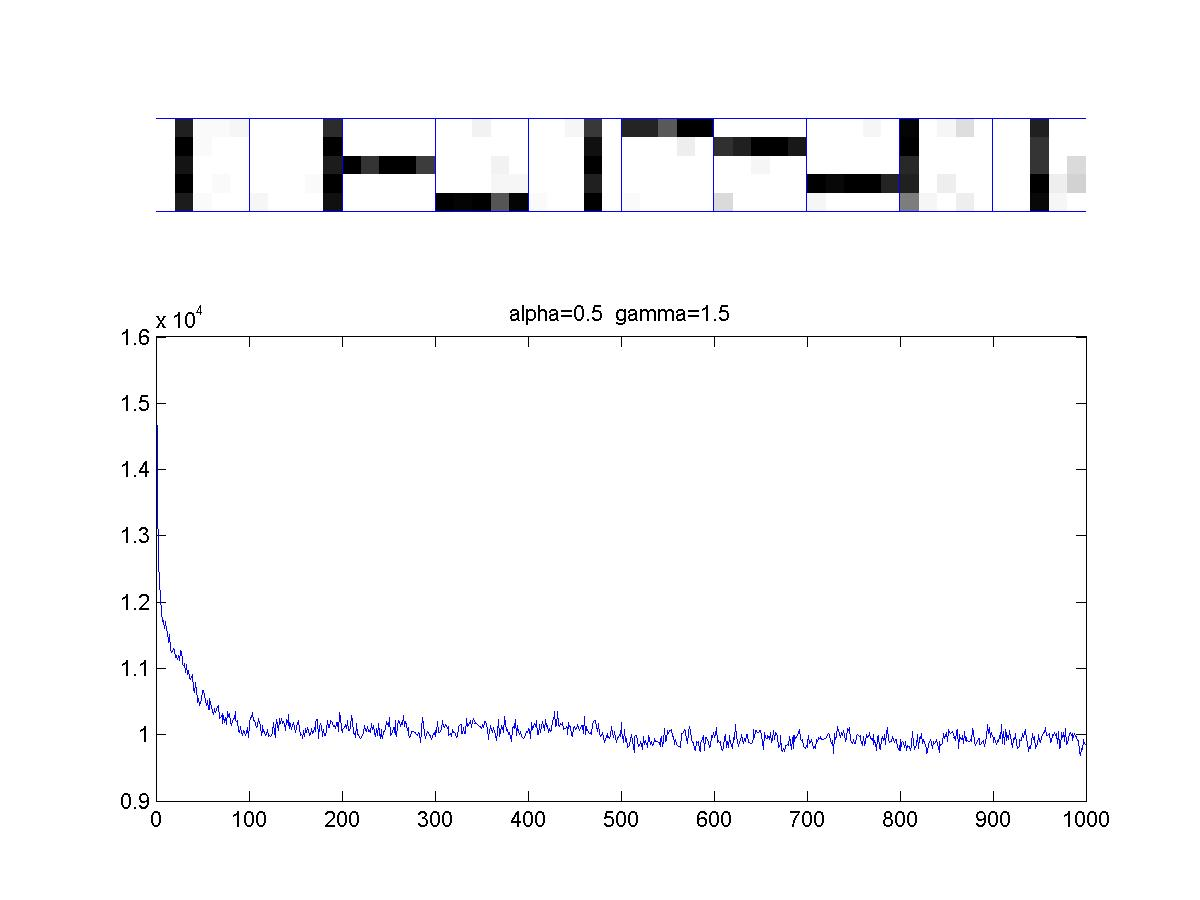
\includegraphics[width=3.5in,height=3in]{exp_gib.jpg} 
    \caption{Gibbs}
    \label{fig:by:table}  
   \end{minipage}% 
\end{figure}

\begin{figure}[h] 
  \begin{minipage}[b]{0.5\textwidth} 
    \centering 
    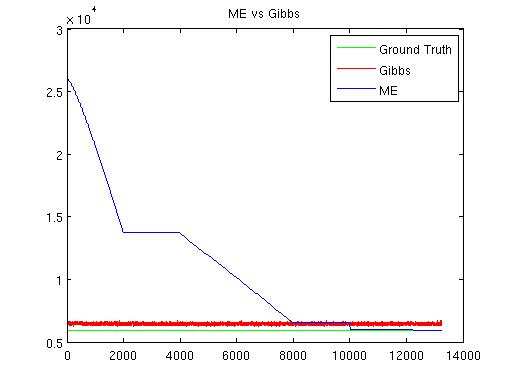
\includegraphics[width=3.5in,height=3in]{hdp_com.jpg} 
    \caption{ME vs Gibbs} 
    \label{fig:by:table} 
  \end{minipage}% 
  \begin{minipage}[b]{0.5\textwidth} 
    \centering 
    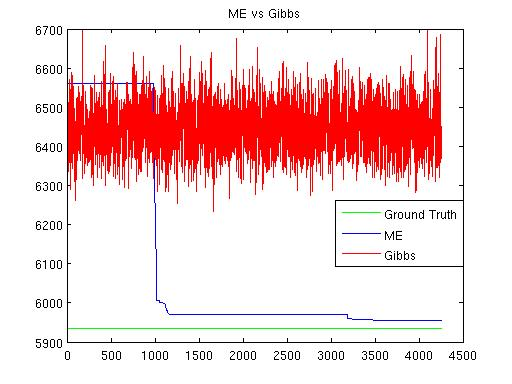
\includegraphics[width=3.5in,height=3in]{hdp_com2.jpg} 
    \caption{ME vs Gibbs}
    \label{fig:by:table}  
   \end{minipage}% 
\end{figure}

\end{spacing}
\end{document}

%%%%%%%%%%%%%%%%%%%%%%%%%%%%%%%%%%%%%%%%%%%%%%%%%%%%%%%%%%%%%
